% !TeX root = ../praktikum.tex
% !TeX encoding = UTF-8
% !Tex spellcheck = de_DE

In diesem Versuchsabschnitt werden die beiden zu untersuchenden Effekte gemessen, während an der Probe ein Gleichstrom anliegt. Hierzu wird gleichzeitig der Spannungsabfall über die Länge und über die Breite der Probe mit der Software erfasst. Angelegt wird ein konstanter Gleichstrom von $\unit[1]{\mu A}$ in x-Richtung an die Probe. Um eine stabile Temperatur zu erhalten wurde die Kammer wieder auf \unit[2]{K} geheizt. Jetzt wurde das Magnetfeld auf \unit[-7]{T} gefahren. Dies dauert rund sieben Minuten, da es sich um supraleitende Spulen handelt und das anlegen eines Stromes eine Gegeninduktion verursacht. Sobald das Magnetfeld aufgebaut ist, wird die Hallspannung $U_H=U_{xx}$ sowie $U_{xy}$ aufgezeichnet während das Magnetfeld mit etwa \unitfrac[1]{T}{min} auf \unit[7]{T} gefahren wird. 


Diese Messdaten sind zusammen mit einer weiteren Messung im Bereich von $-2$ bis \unit[+2]{T} in Abbildung~\ref{fig:full_range_dc} aufgetragen.

\begin{figure}[h]
	\centering
	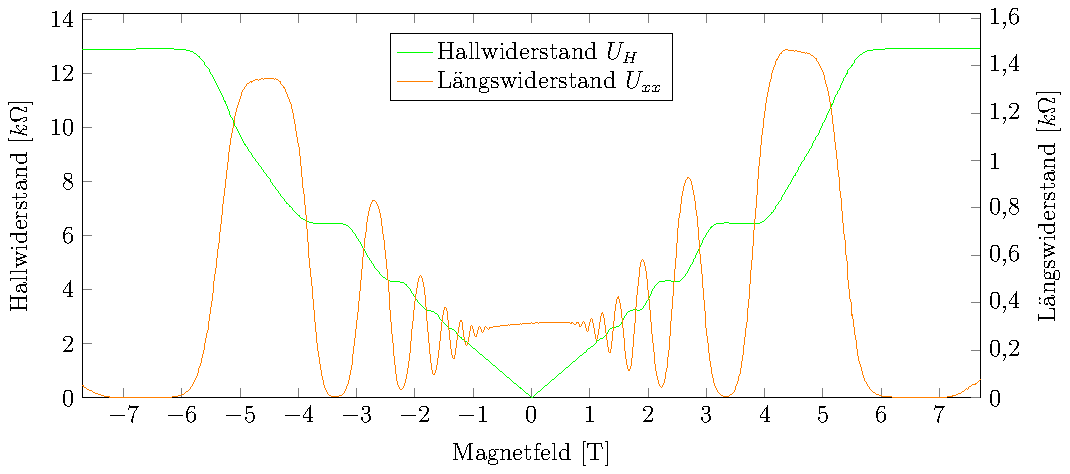
\includegraphics{graphs/dc/full_range.pdf}
	\caption[Gleichstrommessung im maximalen Magnetfeldbereich]{
		Hall-Widerstand und Shubnikov-de Haas Oszillationen eines mit Gleichstrom durchflossenen 2DES.
	}
	\label{fig:full_range_dc}
\end{figure}

Es sind deutlich die Plateaus des Hall- und Shubnikov-de Haas-Widerstandes zu erkennen.